\setcounter{section}{15}


\section{Lecture 16: Feb 24}


\subsection*{Last time}
\begin{itemize}
 \item Dummy-Variable regression (JF chapter 7)
 \item Interactions
\end{itemize}


\subsection*{Today}
\begin{itemize}
 \item Unusual and influential data (JF chapter 11)
\end{itemize}

\subsection*{Unusual and influential data}

Linear models make strong assumptions about the structure of data, assumptions that often do not hold in applications.
The method of least squares can be very sensitive to the structure of the data and may be markedly influenced by one or a few unusual observations.

\subsubsection*{Outliers}
In simple regression analysis, an \underline{outlier} is an observation whose response-variable value is {\it conditionally} unusual {\it given} the value of the explanatory variable: see Figure~\ref{fig:outlier}.
%
\begin{figure}[H]
\begin{center}
  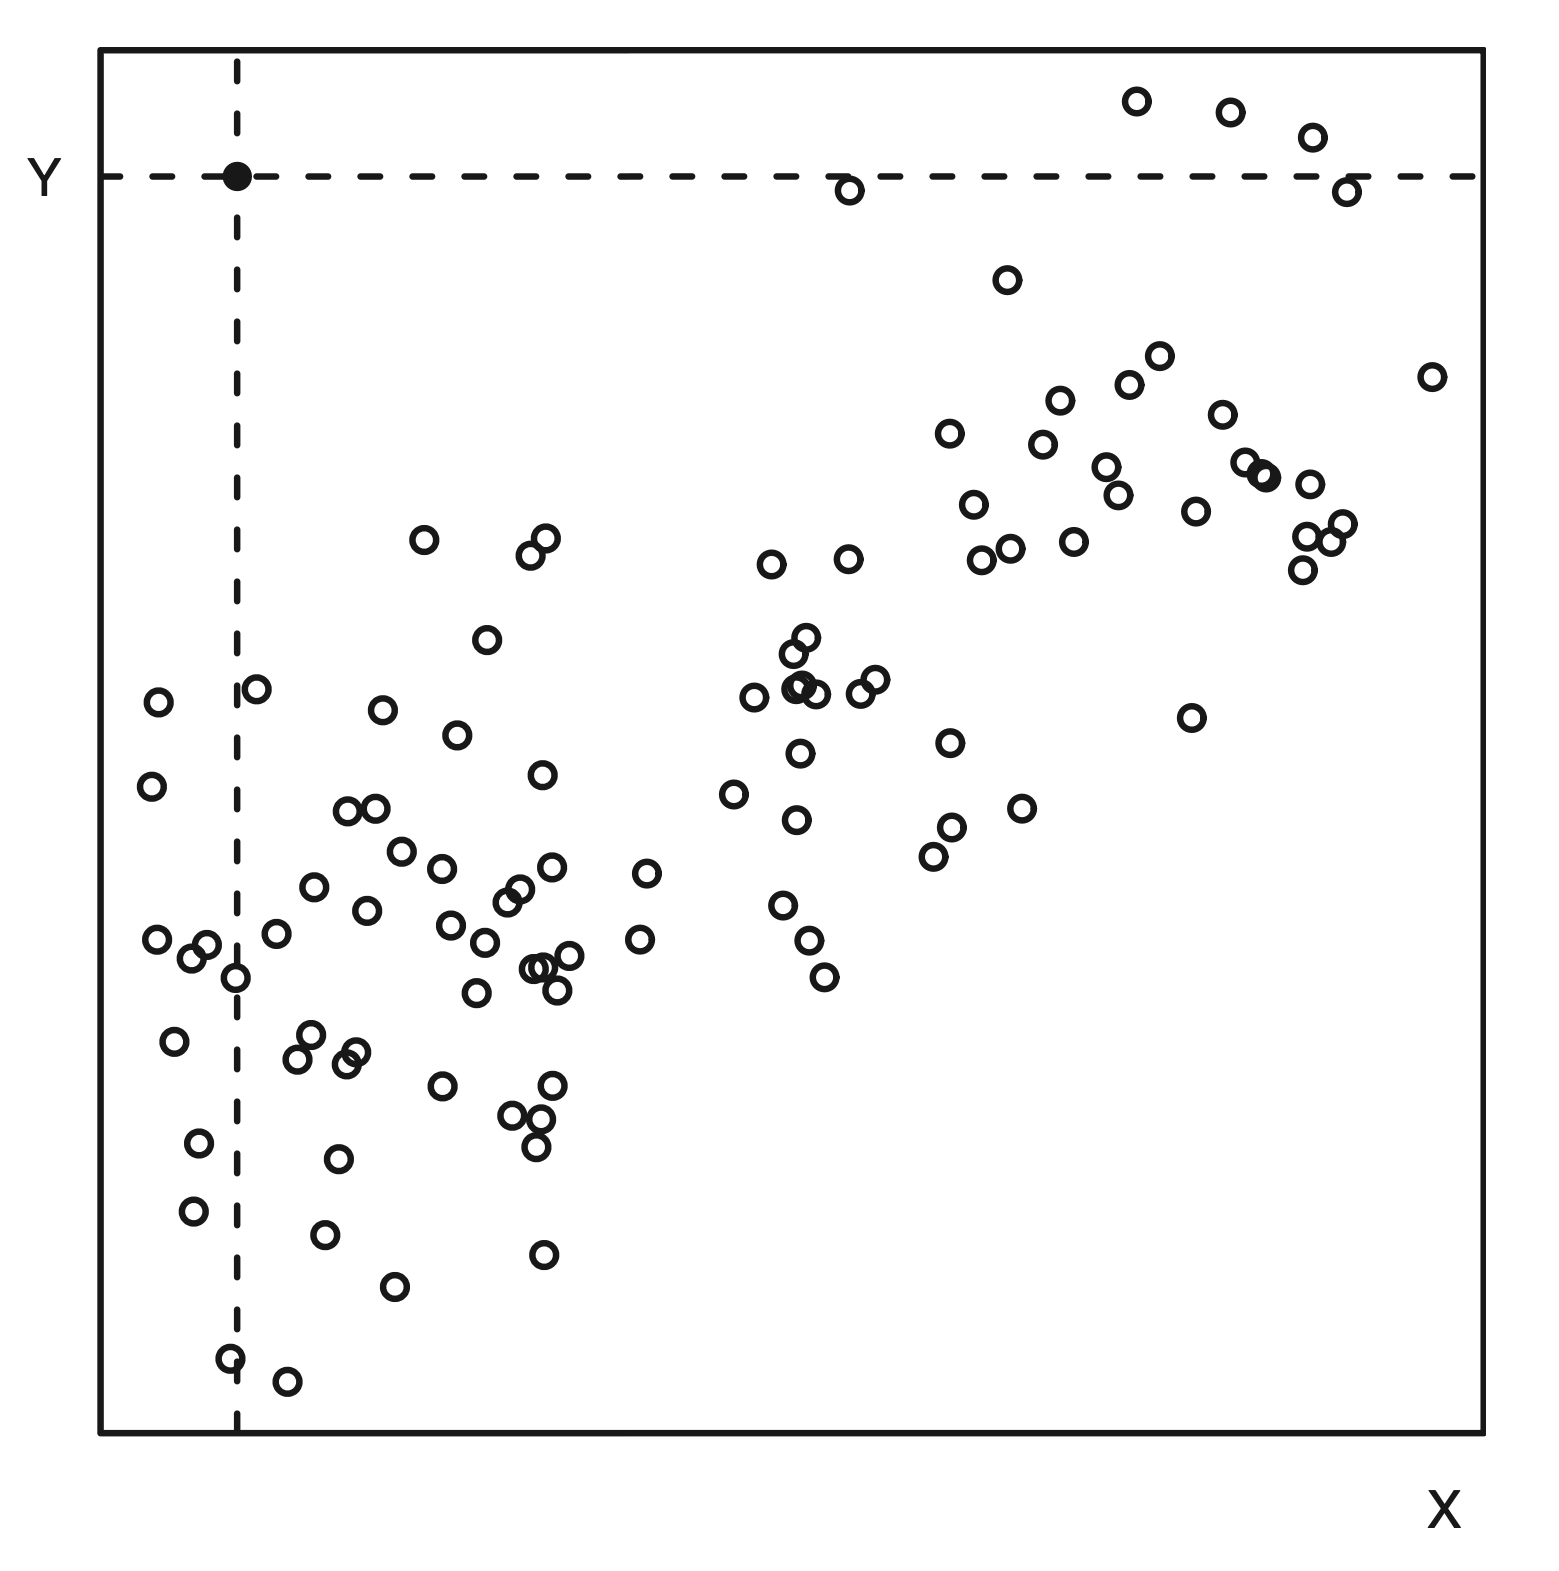
\includegraphics[width=0.4\textwidth]{Lecture16/JF_11_1}
  \caption{The black point is a regression outlier because it combines a relatively large value of $Y$ with a relatively small value of $X$, even though neither its $X$-value nor its $Y$-value is unusual individually.
  Because of the positive relationship between $Y$ and $X$, points with small $X$-values also tend to have small $Y$-values, and thus the black point is far from other points with similar $X$-values.
   JF Figure 11.1.}
  \label{fig:outlier}
\end{center}
\end{figure}
%

Unusual data are problematic in linear models fit by least squares because they can unduly influence the results of the analysis.
Their presence may be a signal that the model fails to capture important characteristics of the data.

Figure~\ref{fig:leverage_and_influence} illustrates some distinctions for the simple-regression model $Y=\beta_0 + \beta_1 X + \epsilon$.
%
\begin{figure}[H]
\begin{center}
  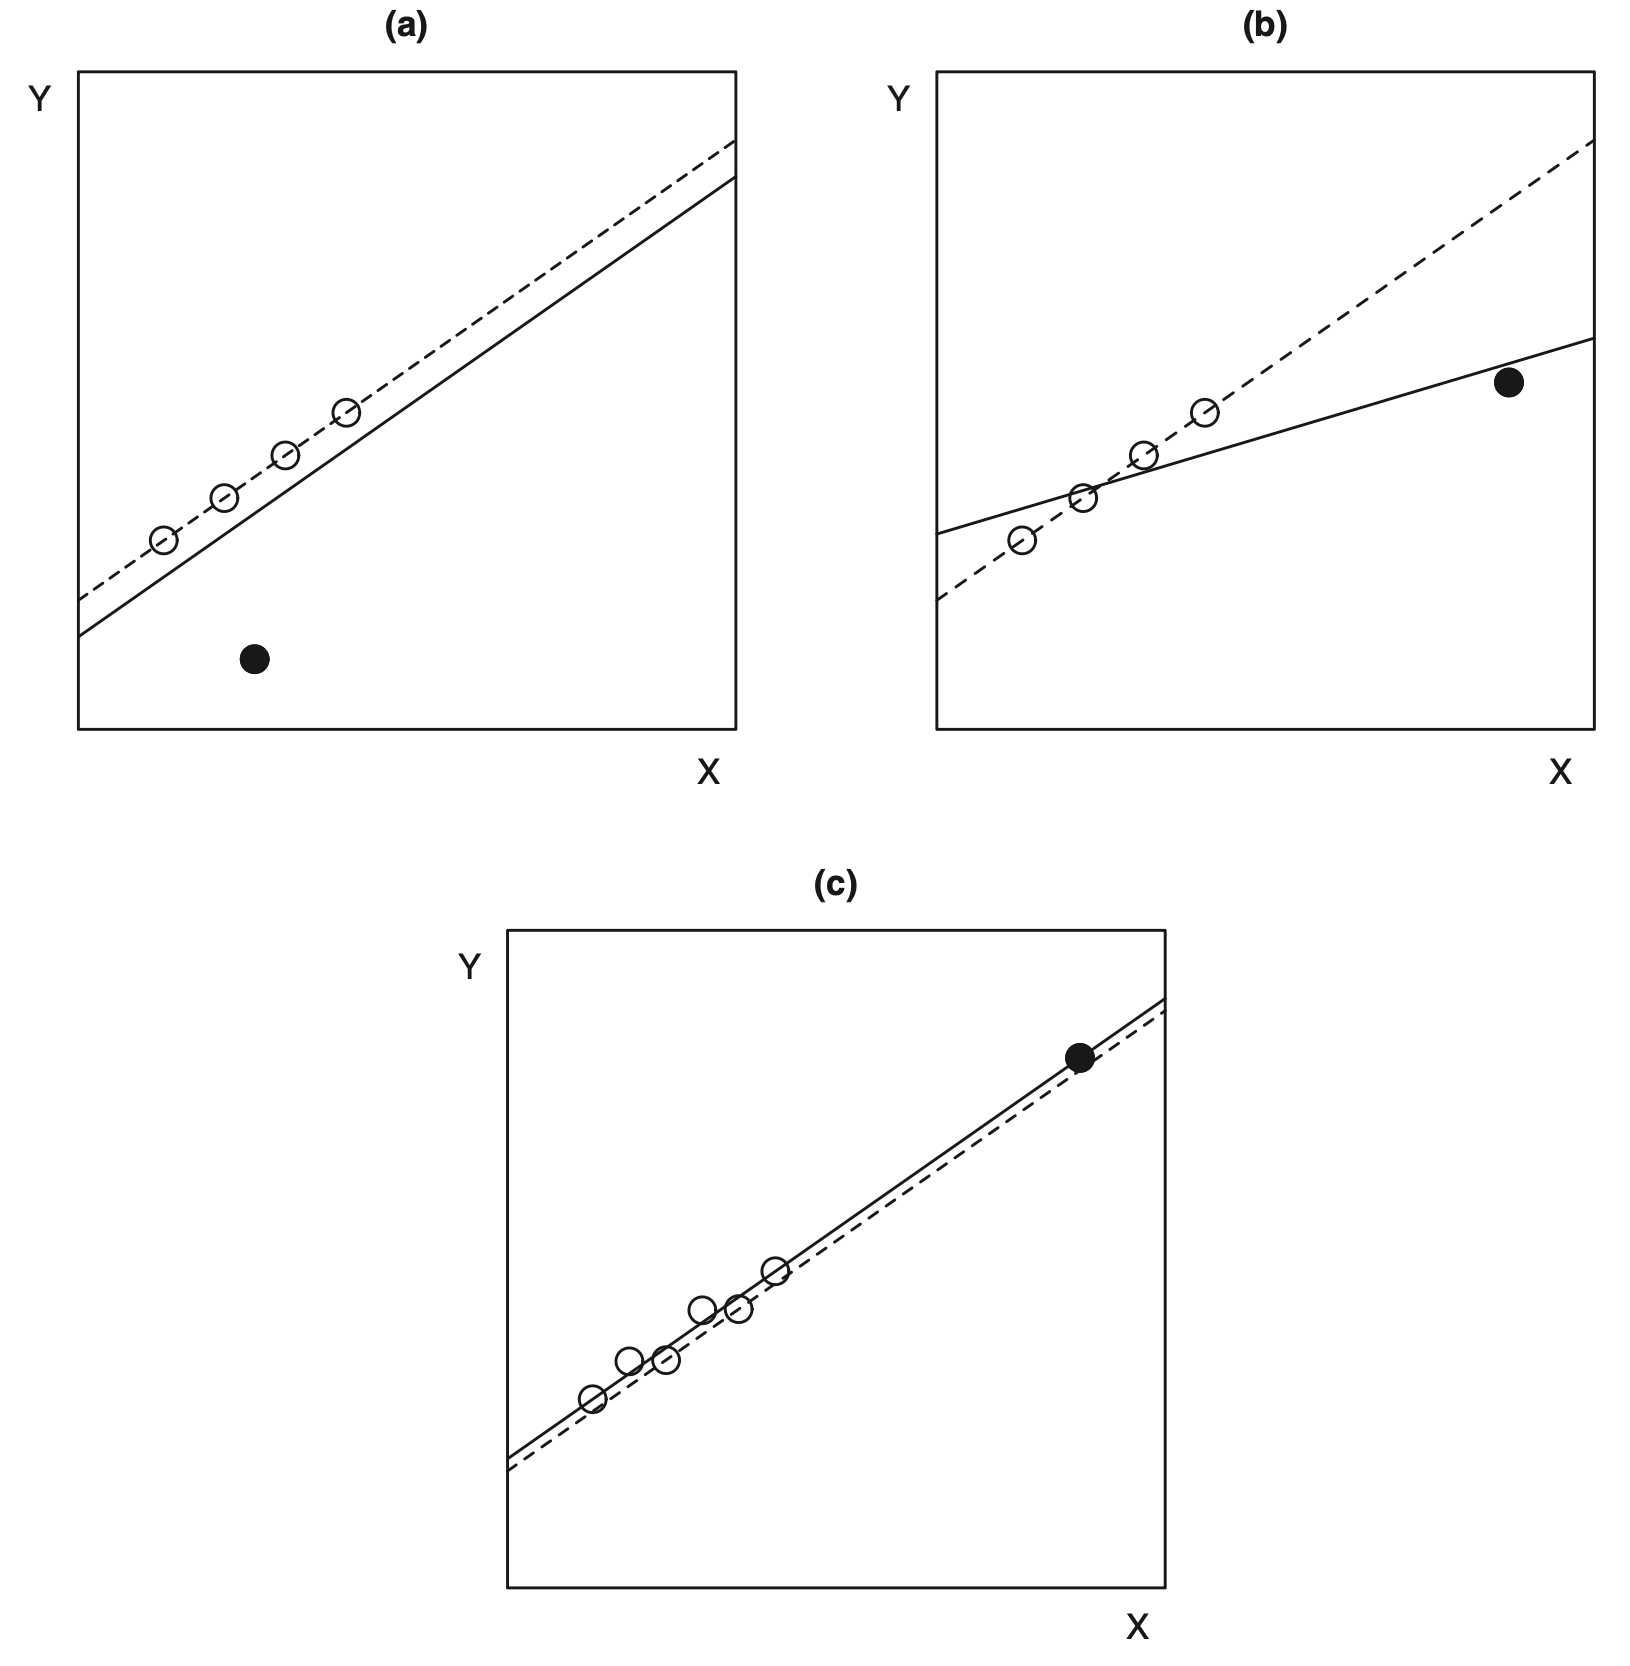
\includegraphics[width=0.8\textwidth]{Lecture16/JF_11_2}
  \caption{Leverage and influence in simple regression.
  In each graph, the solid line gives the least-squares regression for all the data, while the broken line gives the least-squares regression with the unusual data point (the black circle) omitted.
  (a) An outlier near the mean of $X$ has low leverage and little influence on the regression coefficients.
  (b) An outlier far from the mean of $X$ has high leverage and substantial influence on the regression coefficients.
  (c) A high-leverage observation in line with the rest of the data does not influence the regression coefficients.
  In panel (c), the two regression lines are separated slightly for visual effect but are, in fact, coincident
   JF Figure 11.2.}
  \label{fig:leverage_and_influence}
\end{center}
\end{figure}
%

Some qualitative distinctions between outliers and high leverage observations:
\begin{itemize}
  \item An \underline{outlier} is a data point whose response $Y$ does not follow the general trend of the rest of the data.
  \item A data point has high \underline{leverage} if it has ``extreme'' predictor $X$ values:
    \begin{itemize}
      \item With a single predictor, an extreme $X$ value is simply one that is particularly high or low.
      \item With multiple predictors, extreme $X$ values may be particularly high or low for one or more predictors, or may be ``unusual'' combinations of predictor values .
    \end{itemize}
\end{itemize}
And the \underline{influence} of a data point is the combination of leverage and discrepancy (``outlyingness'') though the following heuristic formula:
$$
\mbox{Influence on coefficients} = \mbox{Leverage} \times \mbox{Discrepancy}.
$$

\subsubsection*{Assessing leverage: hat-values}
The \underline{hat-value} $h_i$ is a common measure of leverage in regression.
They are named because it is possible to express the fitted values $\hat{Y}_j$ (``Y-hat'') in terms of the observed values $Y_i$:
$$
\hat{Y}_j = h_{1j} Y_1 + h_{2j} Y_2 + \dots + h_{jj} Y_j + \dots + h_{nj} Y_n = \sum\limits_{i = 1}^n h_{ij} Y_i.
$$
The weight $h_{ij}$ captures the contribution of observation $Y_i$ to the fitted value $\hat{Y}_j$: If $h_{ij}$ is large, then the $i$th observation can have a considerable impact on the $j$th fitted value.
With the least square solutions, for the fitted values:
$$
\hat{\vecc{Y}} = \vecc{X\beta} = \vecc{X} (\vecc{X}\transpose \vecc{X})^{-1} \vecc{X}\transpose \vecc{Y}
$$
we (already) get the \underline{hat matrix}:
$$
\vecc{H} = \vecc{X} (\vecc{X}\transpose \vecc{X})^{-1} \vecc{X}\transpose
$$

{\it Properties:}
\begin{itemize}
  \item (idempotent) $\vecc{H} = \vecc{HH}$
  \item $h_i \equiv h_{ii} = \sum_{j = 1}^n h_{ij}^2$
  \item $\frac{1}{n} \le h_{i} \le 1$    (\href{https://www.ine.pt/revstat/pdf/rs160104.pdf}{a proof} by Mohammad Mohammadi)
  \item $\bar{h} = (p + 1) / n$
\end{itemize}

In the case of SLR, the hat-values are:
$$
h_i = \frac{1}{n} + \frac{(X_i - \bar{X})^2}{\sum_{j = 1}^n (X_j - \bar{X})^2}
$$

\subsubsection*{Detecting outliers: studentized residuals}
The variance of the residuals ($\hat{\epsilon}_i = Y_i - \hat{Y}_i$) do not have equal variances (even if the errors $\epsilon_i$ have equal variances):
$$
\sVar(\hat{\epsilon}) = \sVar(\vecc{Y - X\hat{\beta}})  = \sVar[(\vecc{I - H})\vecc{Y}]= (\vecc{I - H}) \sVar(\vecc{Y})(\vecc{I - H}) = \sigma^2 (\vecc{I - H})
$$
so that for $\hat{\epsilon}_i$,
$$
\sVar(\hat{\epsilon}_i) = \sigma^2 (1 - h_i).
$$
High-leverage observations tend to have small residuals (in other words, these observations can pull the regression surface toward them).

The \underline{standardized residual} (sometimes called \underline{internally studentized residual})
$$
\hat{\epsilon}_i^{'} \equiv \frac{\hat{\epsilon}}{\hat{\sigma}\sqrt{1 - h_i}}
$$
, however, does not follow a $t$-distribution, because the numerator and denominator are not independent.

Suppose, we refit the model deleting the $i$th observation, obtaining an estimate $\hat{\sigma}_{(-i)}$ of $\sigma$ that is based on the remaining $n-1$ observations.
Then the \underline{studentized residual} (sometimes called \underline{externally studentized residual} )
$$
\hat{\epsilon}_i^{*}  \equiv \frac{\hat{\epsilon}}{\hat{\sigma}_{(-i)} \sqrt{1 - h_i}}
$$
has an independent numerator and denominator and follows a $t$-distribution with $n-p-2$ degrees of freedom.

The studentized and the standardized residuals have the following relationship (Beckman and Trussell, 1974):
$$
\hat{\epsilon}_i^{*} = \hat{\epsilon}_i' \sqrt{ \frac{n - p -2}{n - p - 1 - \hat{\epsilon}_i'^{2}}}
$$

For large $n$,
$$
\hat{\epsilon}_i^{*} \approx \hat{\epsilon}_i' \approx \frac{\hat{\epsilon}}{\hat{\sigma}}
$$

\subsubsection*{Test for outlier}
It is of our interest to pick the studentized residual $\hat{\epsilon}_{max}^{*}$ with the largest absolute value among $\hat{\epsilon}_1^{*}, \hat{\epsilon}_2^{*}, \dots, \hat{\epsilon}_n^{*}$ to test for outlier.
However, by doing so, we are effectively picking the biggest of $n$ test statistics such that it is not legitimate simply to use $t_{n - p - 2}$ to find a $p$-value.
We need a correction on the $p$-value because of multiple-comparisons.

Suppose that we have $p' = \Pr(t_{n - p - 2} > |\hat{\epsilon}_{max}^{*}|)$, the $p$-value before correction.
Then the Bonferroni adjusted $p$-value is $p = n p'$.


\subsubsection*{Measuring influence}
Influence on the regression coefficients combines leverage and discrepancy.
The most direct measure of influence simply expresses the impact on each coefficient of deleting each observation in turn:
$$
D_{ij} = \hat{\beta}_j - \tilde{\beta}_{j(-i)} \quad \mbox{for } i=1, \dots, n \mbox{ and } j=0, 1, \dots, p
$$
where $\hat{\beta}_j$ are the least-squares coefficients calculated for all the data, and the $\tilde{\beta}_{j(-i)}$ are the least-squares coefficients calculated with the $i$th observation omitted.
To assist in interpretation, it is useful to scale the $D_{ij}$ by (deleted) coefficient standard errors:
$$
D_{ij}^* = \frac{D_{ij}}{\reallywidehat{SE}_{(-i)} (\tilde{\beta}_{j(-i)})}
$$
Following Belsley, Kuh, and Welsh (1980), the $D_{ij}$ are often termed DFBETA$_{ij}$, and $D_{ij}^*$ are called DFBETAS$_{ij}$.
One problem associated with using $D_{ij}$ or  $D_{ij}^*$ is their large number $n(p+1)$ of each.

Cook's distance calculated as
$$
D_i = \frac{\sum_{j = 1}^n(\tilde{y}_{j(-i)} - \hat{y}_j )^2}{(p + 1) \hat{\sigma}^2 } = \frac{\hat{\epsilon}_i^{'2} }{p + 1} \times \frac{h_i}{1 - h_i}
$$
In effect, the first term in the formula for Cook's $D$ is a measure of discrepancy, and the second is a measure of leverage.
We look for values of $D_i$ that stand out from the rest.

A similar measure suggested by Belsley et al. (1980)
$$
\mbox{DFFITS}_i = \hat{\epsilon}_i^{*} \frac{h_i}{1 - h_i}
$$
Except for unusual data configurations, Cook's $D_i \approx \mbox{DFFITS}_i^2/(p + 1)$.

\subsubsection*{Numerical cutoffs (suggested)}

\begin{center}
\begin{tabular}{ c c}
\hline
Diagnostic statistic & Cutoff value\\
\hline
$h_i$ & $ 2 \bar{h} =  \frac{2(p + 1)}{n}$, ($3\bar{h}$ for small sample)\\
$D_{ij}^*$ & $|D_{ij}^*| > 1$ or $2$ ($2/\sqrt{n}$ for large samples)\\
Cook's $D_i$ & $D_i > \frac{4}{n - p -1}$\\
$\mbox{DFFITS}$ & $|\mbox{DFFITS}_i| > 2 \sqrt{ \frac{p + 1}{n - p - 1}}$ \\
\hline
\label{table:distributions}
\end{tabular}
\end{center}







